\documentclass{rapportCS}
\usepackage{lipsum}
\usepackage[utf8]{inputenc}
\usepackage{amsmath}
\usepackage{amsfonts}
\usepackage{stmaryrd} % more math symbols
\usepackage{amsthm} % for theoreme style
\usepackage{graphics}
\usepackage{algorithm,algorithmic}
\usepackage{caption}
\usepackage{mathtools}
\newlength\myindent
\setlength\myindent{2em}
\newcommand\bindent{%
  \begingroup
  \setlength{\itemindent}{\myindent}
  \addtolength{\algorithmicindent}{\myindent}
}
\newcommand\eindent{\endgroup}

%%%% for images
\usepackage{graphicx}

\title{Rapport ECS Template} %Titre du fichier

\begin{document}

%----------- Informations du rapport ---------
\titre{
{\LARGE \bfseries \textit{Tsunami propagation using neural networks}\\[0.1cm] }} %Titre du fichier .pdf

\enseignant{ Frédéric \textsc{Magoulès}\\Joanna \textsc{Tomasik}
}%Nom de l'enseignant


\eleves{Lawson \textsc{Oliveira Lima}\newline
        Julien \textsc{Rosenberger} \newline
        Antier \textsc{Esteban} \newline
        Besbes \textsc{Mariem} \newline
        Paun \textsc{Théodore} \newline
        Ruault \textsc{Gabriel} \newline
        } %Nom des élèves


%----------- Initialisation -------------------
        
\fairemarges%Afficher les marges
\fairepagedegarde%Créer la page de garde
\tabledematieres%Créer la table de matières


%====================== INCLUSION DES PARTIES ======================
%régler l'espacement entre les lignes
\newcommand{\HRule}{\rule{\linewidth}{0.5mm}}

%recommencer la numérotation des pages à "1"

\chapter{Introduction }\label{ch:Introduction}
\section{Context and objectifs}\label{sec:Contexte}
Tsunamis do not occur very often but are devastating phenomena. Research
and studies about tsunamis try to predict the impact of such events to protect
people. Due to the sheer scale of tsunami, laboratory and analytical models are
not relevant. The former because we can not obtain an equivalent scale model
in a lab, the latter because there is no analytical solution to the propagation
equations. Although a numerical resolution can approximate the solution, it
requires a huge computing power and time without taking into account the accuracy errors due to turbulence phenomena. 

\section{State of the art}\label{sec:Contexte}



\section{Contribution}\label{sec:Contribution}


\section{Report Structure}\label{sec:Contribution}
First, it is presented how important and effective this approach is, then
the second chapter shows basic concepts about a neural network and its behavior, as well as a brief introduction to differential equations.
Then in the third paragraph we explain our approche and solve some partial differential equations using neural networks.
After that, in the fifth paragraph, the describes how obtain the domain to do the Tsunami simulation, that is, the mesh to make the simulation.

\chapter{Concepts}\label{ch:2}
\section{Neural networks}
Now the basis of multiple state of the art technologies in data science, neural networks provide a framework we hope can solve propagation equations in a shorter time than with regular finite elements.\\
For now, we will focus on the study of multilayer perceptron, one of the first neural networks to have been developped. They consist in an input layer, a vector of $n$ components, and an output layer, of $p$ components.
The input is subjected to a series of linear operations and non-linear activations are applied trough "hidden layers" to get the output.\\
A multilayer perceptron can then be seen as a non linear function:
    $$\mathcal{N} : \mathbb{K}^n \rightarrow \mathbb{K}^p$$
\newline
If we note $g_i$ the (non-linear) activation function, and $W_i$ and $b_i$ the weight and bias matrix of the ith hidden layer, then, for a MP with k hidden layers:
\begin{equation}
     \forall x \in \mathbb{K}^n, \mathcal{N}(x) = g_k(b_k + W_k g_{k-1}(b_{k-1}+W_{k-1} g_{k-2}(\dots(b_1 + W_1 x))))
\end{equation}
Through training epoch, passes through the training dataset coupled with gradient descent, we want $\mathcal{N}$ to approach a function of interest.

\section{Partial Differential Equation}
Our goal is to solve the propagation equation of a tsunami, which is a partial differential equation (PDE). In a general sense, a PDE is defined as:
\begin{equation*}
    (E): 
    \begin{cases}
        \mathcal{Q}(u, \nabla u, H u, \dots)(x) = 0 & \text{inside $\Omega$}\\
        \mathcal{R}(u, \nabla u, H u, \dots)(x) = f(x) & \text{on $\partial \Omega$}
    \end{cases}
\end{equation*}

Where $\mathcal{Q}$ and $\mathcal{R}$ are linear operators, $\Omega$ is the domain considered,\\
and $u : \mathbb{K}^n \rightarrow \mathbb{K}^p$ is the solution to $(E)$.\\

Our goal is to replace $u$ with a neural network $\mathcal{N}$ and train it to get a solution to $(E)$.
However, this would mean training on both the domain and its boundary. To avoid this case as the boundary is always defined with boundary conditions, we reformulate the problem:\\

Instead we replace $u$ with $\Psi$ defined as:
\begin{equation}
    \Psi(x) = A(x) + F(x)\mathcal{N}(x)
\end{equation}
Where $A$ verifies the boundary conditions, and $F$ is null on the boundary.\\
As such, we unconstrained the problem, and the neural network can train inside the domain, with the boundary conditions handled by the above mentionned functions.




\section{Find A}
In this section we propose two choices for the function $A$ in 2 different contexts.\\
Let $K$ be a point in space with coordinates 
\begin{math}
\Vec{x_K} = \sum x_j\Vec{e_j}
\end{math}

\subsection{Function 1}
\begin{equation*}
    \forall x \in \mathbb{R}^k, \psi_K(x)=
    \left\{
    \begin{matrix}
    \exp \left( -\frac{1}{l^2 - d(x,K)^2} \right) & if \ d(x,K)^2<l^2\\
    0 & else
    \end{matrix}
    \right\}
\end{equation*}
Where 
\begin{math}
    d(x,K)^2 = \lVert x - x_K \rVert^2
\end{math}
\newline
This function has the advantage of not interacting with the space located beyond a distance $l$ away from point $A$

\subsubsection{Use in our case}
Let $\Omega$ be a domain, and $\partial\Omega$ its boundary. We sample $N$ points from the boundary with coordinates $x_i$ such as $g(x_i)=g_i$. Let us use 
\[
l = \min_{1\leq i,j \leq N}\lVert x_i - x_j \rVert
\]
\newline
Then, we can use the following function to compute the value of the boundary with interesting properties.
\begin{equation*}
    \Psi(x) = \exp \left( \frac{1}{l^2} \right) \sum_{i=1}^{N}g_i\psi_i(x)
\end{equation*}

\subsubsection{Boundary conditions} 
We do verify the boundary conditions:
\begin{equation*}
    If \ x=x_j\in \partial \Omega, \Psi(x_j) = g_j
\end{equation*}

As by hypothesis, for $\psi_j$ the distance is null, and for all other $\psi_i$ we are at a distance greater than $l$ away from $x_i$.

\subsubsection{Regularity}
By summing $\psi$ functions, we have that $\Psi$ is a class $C^\infty$ function.

\subsubsection{Derivative}
By using chain rule, we can easily calculate the derivative according to any variable j with
\begin{equation*}
    \partial_j \Psi(x) = \exp\left(\frac{1}{l^2}\right)\sum_{i=1}^{N}g_i\partial_j\psi_i(x)
\end{equation*}
and
\begin{equation*}
    \partial_j\psi_i(x) = \frac{-2(x_j-x_{Aj})}{(l^2 - d(x,i)^2)^2}\psi_i(x)
\end{equation*}

\subsubsection{Bounded function}
By definition, we have
\begin{equation*}
    \forall x \in \mathbb{R}^k, \min_{1 \leq i \leq N}g_i \leq \Psi(x) \leq \max_{1 \leq i \leq N}g_i
\end{equation*}

\subsubsection{Ease of computation}
To calculate $\Psi$ and its gradient, a lot of elements are redundant and thus can be evualated once, like $l$ (when we sample the boundary) and $l^2-d(x,i)^2$ for each point of the boundary.

\subsubsection{Issues}
This function is too restrictive to be usable in practice. With too much sample boundary points, this function becomes a series of spikes, and thus does not approximate the boundary asymptotically.\\
In case of a small amount of samples, this function is useful.

\subsection{Function 2}
\begin{equation*}
    \forall x \in \mathbb{R}^k, \psi_K(x)= 1 - \tanh \left( \frac{d(x,K)}{l} \right)^2
\end{equation*}

This time with:
\begin{equation*}
    \Psi(x) = 0.5 \sum_{i=1}^{N}g_i\psi_i(x)
\end{equation*}

This time, our function verifies the boundary conditions only asymptotically with a uniformly sampled boundary.\\
The $0.5$ coefficient is their to correct for the first order interactions between two adjacent $\psi_K$.\\
Through numerical simulations, we obtain a smoothed boundary that closely ressembles the real boundary with enough sample points.
In our simulation, this function will be mostly used as the $A$ function.

\section{Find F}
Set $(d,n)\in \mathbb{N}^*$ and $(x_i)_{i\in \llbracket0;n-1\rrbracket }\in \mathbb{R}^{d}$ distinct one another. We seek a polynomial $F\in\mathbb{K}[X]$ such that $\mathbb{K} \in \{\mathbb{R},\mathbb{C}\}$ and
$$\forall i\in \llbracket1;n\rrbracket,~F(x_i)=0 \text{ and } \exists x_n:~F(x_n)\neq0$$

\subsection{Case 1D}
In the case $d=1$, Vandermonde polynomials are a good start. The only thing to add to the construction is a point where the polynomial $F$ is not null. Assuming the orthobarycentre of the family $(x_i)_{i\in \llbracket0;n-1\rrbracket }$ is not already inside, let's take the orthobarycentre of these points defined as $x_n:=\frac{1}{n}\sum_{i=0}^{n-1} x_i$.\\
The system induced is this one :
\begin{equation*}
    \begin{pmatrix}
        1 & x_0 & \dots & x_{0}^{n} \\
        \vdots & \vdots & \ddots & \vdots\\
        1 & x_{n-1} & \dots & x_{n-1}^{n} \\
        1 & x_n & \dots & x_n^{n-1} 
    \end{pmatrix}
    \begin{pmatrix}
        a_0\\
        \vdots\\
        a_{n-1}\\
        a_{n}
    \end{pmatrix}
    =
    \begin{pmatrix}
        0\\
        \vdots\\
        0\\
        1
    \end{pmatrix}
\end{equation*}
that one can solve thanks to the inversion of the Vandermonde matrix, which is non-singular since all the points are distinct one another thanks to the assumption.


\subsection{Case 2D}
The work done here for $d=2$ is meant to be easily generalizable to even greater values of $d$.
Set $\forall i \in \llbracket0;n-1\rrbracket, x_i \text{ has as coordinates }(x_{i,0},x_{i,1})$.

\subsubsection{Matrix method}
\subsubsection*{Start of an idea (inspired from Vandermonde matrix in 1D)}
Globally, $F$ can be defined in $\mathbb{R}_{n+1}[X]$ considering its roots $(x_i)_{i\in \llbracket0;n-1\rrbracket }$ and the point $x_n$ where it is not null. Therefore, set $x_n$ the orthobarycentre with the same assumption as previously 	and $(\alpha_{ij})_{\{(i,j)\in\mathbb{N}:i+j\leq n\}}\in\mathbb{R}^{2n}$ such that
\begin{equation*}
    \forall (x,y) \in \mathbb{R}^2,~F(x) = \sum_{\{(i,j)\in\mathbb{N}:i+j\leq n\}} \alpha_{ij}x^iy^j
\end{equation*}
\begin{equation*}
    \begin{pmatrix}
        1 & x_{0,0} & x_{0,1} & x_{0,0}x_{0,1} & \dots & x_{0,1}^{n} \\
        \vdots & \vdots&\vdots & \vdots& \ddots & \vdots \\
        1 & x_{n-1,0} & x_{n-1,1} & x_{n-1,0}x_{n-1,1} & \dots &x_{n-1,1}^{n} \\
        1 & x_{n,0} & x_{n,1} & x_{n,0}x_{n,1} & \dots & x_{n,1}^{n} \\
    \end{pmatrix}
    \begin{pmatrix}
        \alpha_{00}\\
        \vdots\\
        \alpha_{0(n-1)}\\
        \alpha_{0n}
    \end{pmatrix}
    =
    \begin{pmatrix}
        0\\
        \vdots\\
        0\\
        1
    \end{pmatrix}
\end{equation*}

Actually, Vandermonde does not give any proof of the non-singularity of the left matrix and one could thought about putting more combinations of the coordinates of each point to extract a non-singular matrix after.
Yet, finding this extracted matrix remains computationally heavy in addition to being uncertain.\\

\subsubsection*{In hindsight}
The realm this idea steps into is the realm of principal component analysis. It remains interesting considering the fast differentiation of the polynomial one could get after. Nevertheless, it could force us to already use machine learning which will require some time to compute accurately and will always remain an approximation of the true solution we seek.




\subsubsection{Direct approach}
In this kind of situation, constructing the polynomial $$F:(x,y)\mapsto\prod_{m=0}^{n-1}(x-x_i)(y-y_i)$$ quickly comes to mind. Nevertheless, $F$ would be to often null on the domain and could induce great errors after. So, the idea is to replace the given factor by one null only at a given point as shown here:
$$\forall (x,y)\in\mathbb{R}^2,~F_r(x,y) = \prod_{k=0}^{n-1}((x-x_k)^2 + (y-y_k)^2)$$
\newline
$$\forall (x,y)\in\mathbb{R}^2,~F_c(x,y) = \prod_{k=0}^{n-1}((x-x_k) + i(y-y_k))$$
\newline
$$\forall (x,y)\in\mathbb{R}^2,~F_s(x,y) = \prod_{k=0}^{n-1}(\sin(x-x_k)\sin(y-y_k))$$

\begin{itemize}
    \item $\forall (x,y)\in\mathbb{R}^2,~F_r(x,y)=\vert F_c(x,y) \vert^2$ and $|~F_s(x,y)|<=1$
    \item the coefficients of $F_c$ are faster to compute but harder to evaluate than the ones of $F_r$
    \item the coefficients of $F_s$ are as fast as $F_c$ to compute and it's bounded, a important characteristical 
\end{itemize}

\chapter{PDEs using neural networks} 
\label{chapter3}
\section{Hyperparameters}
Here is the scheme of model tuning followed:
\begin{figure}[h]
    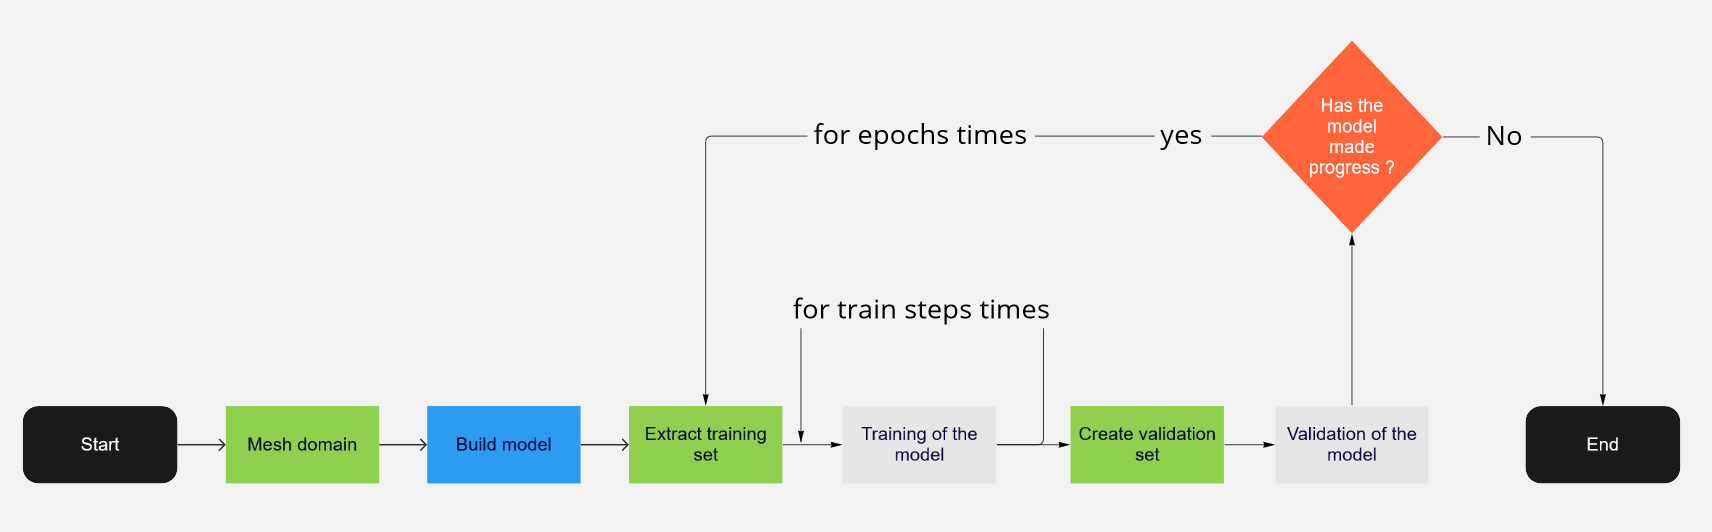
\includegraphics[width=13cm, height=4cm]{images/tuning_model.png}
    \centering
    \caption{scheme of a model tuning}
\end{figure}

The red box involves using an early stopping callback to stop the epoch loop when the model begins to overfit. A \texttt{patience} integer set how far the system will go back in history. If during \texttt{patience} epochs the has not made progress the epoch loop is stopped.
\newline
The hypertuning comes when one wants to construct a model and a training that will end to a low validation error. Let's list all the hyperparameters involved in this scheme applied for the Poisson equation on a square domain:
\begin{itemize}
    \item \texttt{grid\_length}: integer setting the number of points in the domain to \texttt{grid\_length}x\texttt{grid\_length}
    \item \texttt{l\_units}: list of integers depicting the number of hidden layers and the number of neurons per layer of the sequential machine learning model
    \item \texttt{l\_activations}: list depicting the activation functions of each layer of the model
    \item \texttt{noise}: integer in $\{0,1\}$ conditioning the use of a Gaussian layer of mean $0$ after the input layer
    \item \texttt{stddev}: the standard deviation of the Gaussian layer when it is used
    \item \texttt{optimizer}: string depicting the optimizer used
    \item \texttt{learning\_rate}: float setting the learning rate of the previous optimizer
    \item \texttt{epochs\_max}: integer setting the number of maximum epoch loops
    \item \texttt{n\_trains}: integer setting the number of train loops
    \item \texttt{batch\_size}: integer setting the number of points extracted from the mesh to construct the training set at each epoch loop
    \item \texttt{patience}: integer setting how many epoch loops the system can go on without progressing, after that the trial is ended
\end{itemize}

An automatization of the hypertuning by hand and using Keras Tuner has already been led. Nevertheless, some work must still be done to assure a low validation error with minimal cost of time and hardware. A few bugs, impeding a proper convergence, also seems to persist in some of our implementations.

\newpage
\section{Pseudo-code}
\label{pseudo_code}
\begin{algorithm}[H]
    \caption*{Algorithm to solve a PDE using neural networks}
    \hspace*{\algorithmicindent} \textbf{Input} a,b,c\\
    \hspace*{\algorithmicindent} \textbf{Output} d
    \begin{algorithmic}
    \STATE a $\leftarrow$ c
    \STATE b $\leftarrow$ a
    \STATE \textbf{function} \quad resursion(a,b)
        \bindent
        \RETURN a
        \eindent
    \end{algorithmic}
    \end{algorithm}

\section{Activation functions}
\label{activation}

\newpage
\section{PDE example}
\label{pde_example}
We want to solve the following PDE using the algorithm described on section \ref{pseudo_code} with some activation functions of the section \ref{activation}.
\begin{equation}
    \Delta \psi(x,y) +\psi(x,y)\cdot\frac{\partial \psi(x,y)}{\partial y}= f(x,y) \quad\text{on}\quad \Omega = [0,1]^2  
\end{equation}
with boundary conditions $\psi(0,y)=\psi(1,y)=\psi(x,0)=0$ and $\frac{\partial \psi}{\partial y}(x,1)=2\sin(\pi x)$           
and $f(x, y)=\sin(\pi x)(2-\pi^2y^2+2y^3\sin(\pi x))$. 
\newline
This problem has a analytical solution $\psi_t$ s.t $\psi_t(x, y)=y^2sin(\pi x)$. Thus, to solve it and compare the results we define our loss function like $\mathcal{L} = ||\Delta \psi_a(x,y) +\psi(x,y)\cdot\frac{\partial \psi(x,y)}{\partial y}-f(x,y) ||_2$  
and the approximated solution like $\psi_a(x,y)=F(x,y)N(x,y)+A(x,y)$ with:
\begin{itemize}
    \item $F(x,y)=\sin(x-1)\sin(y-1)\sin(x)\sin(y)$
    \item $A(x,y)=y\sin(\pi x)$        
\end{itemize}

\section{Jax approach}
\subsection{Jax library}
Jax is a python library built using NumPy and the lax architecture, which makes it high performance and highly recommended for simulations that have a high computational cost. Also, because of the way it is used to implement a neural network, it is possible to parallelize several steps of the simulation so that it runs faster.  
Therefore, due to these characteristics, we chose to do some tests with it.

\subsection{Solving with tanh}
On the image below we can see the results obtained for the PDE of the section \ref{pde_example} using $\tanh$.
\begin{figure}[H]
\begin{subfigure}{0.45\textwidth}
    \centering
    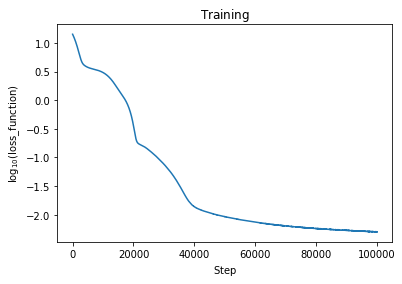
\includegraphics[width=.8\linewidth]{images/NN_Jax_PDE8_files_tanh/NN_Jax_PDE8_18_1.png}
    %\caption{A subfigure}
    \label{fig:sub1}
\end{subfigure}%
\begin{subfigure}{0.45\textwidth}
    \centering
    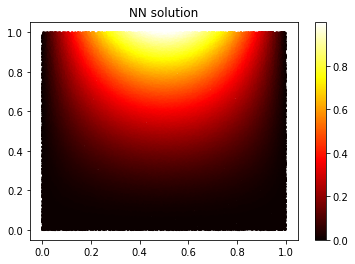
\includegraphics[width=0.8\linewidth]{images/NN_Jax_PDE8_files_tanh/NN_Jax_PDE8_20_0.png}
    %\caption{A subfigure}
    \label{fig:sub2}
\end{subfigure}
\newline
\begin{subfigure}{.45\textwidth}
    \centering
    \includegraphics[width=.8\linewidth]{images/NN_Jax_PDE8_files_tanh/NN_Jax_PDE8_22_0.png}
    %\caption{A subfigure}
    \label{fig:sub3}
    \end{subfigure}
\begin{subfigure}{.45\textwidth}
    \centering
    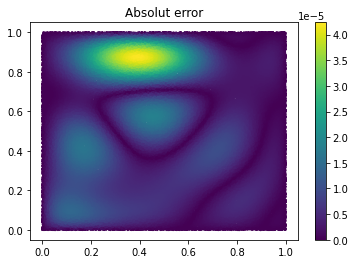
\includegraphics[width=.8\linewidth]{images/NN_Jax_PDE8_files_tanh/NN_Jax_PDE8_24_0.png}
    %\caption{A subfigure}
    \label{fig:sub4}
\end{subfigure}
\caption{Results using Jax and tanh}
\label{fig:test}
\end{figure}

\newpage
\subsection{Solving with sigmoid}
On the image below we can see the results obtained for the PDE of the section \ref{pde_example} using sigmoid.
\vspace{-0.85cm}
\begin{figure}[H]
\begin{subfigure}{.45\textwidth}
    \centering
    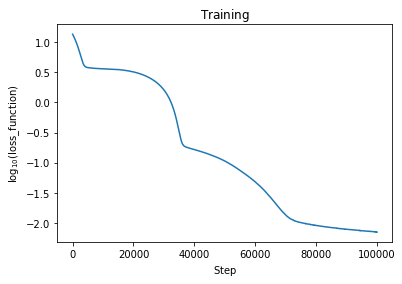
\includegraphics[width=.8\linewidth]{images/NN_Jax_PDE8_files_sigmoid/NN_Jax_PDE8_18_1.png}
    %\caption{A subfigure}
    \label{fig:sub1}
\end{subfigure}%
\begin{subfigure}{0.45\textwidth}
    \centering
    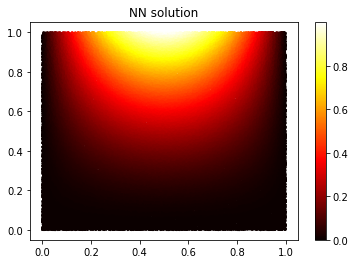
\includegraphics[width=0.8\linewidth]{images/NN_Jax_PDE8_files_sigmoid/NN_Jax_PDE8_20_0.png}
    %\caption{A subfigure}
    \label{fig:sub2}
\end{subfigure}
\newline
\begin{subfigure}{.45\textwidth}
    \centering
    \includegraphics[width=.8\linewidth]{images/NN_Jax_PDE8_files_sigmoid/NN_Jax_PDE8_22_0.png}
    %\caption{A subfigure}
    \label{fig:sub3}
    \end{subfigure}
\begin{subfigure}{.45\textwidth}
    \centering
    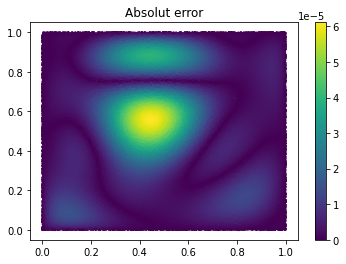
\includegraphics[width=.8\linewidth]{images/NN_Jax_PDE8_files_sigmoid/NN_Jax_PDE8_24_0.png}
    %\caption{A subfigure}
    \label{fig:sub4}
\end{subfigure}
\caption{Results using Jax and sigmoid}
\label{fig:test}
\end{figure}

\vspace{-0.5cm}
\subsection{Solving with elu}
On the image below we can see the results obtained for the PDE of the section \ref{pde_example} using elu.
\vspace{-0.45cm}
\begin{figure}[H]
\begin{subfigure}{.45\textwidth}
    \centering
    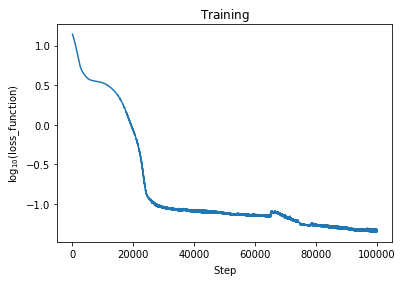
\includegraphics[width=.8\linewidth]{images/NN_Jax_PDE8_files_elu/NN_Jax_PDE8_18_1.png}
    %\caption{A subfigure}
    \label{fig:sub1}
\end{subfigure}%
\begin{subfigure}{0.45\textwidth}
    \centering
    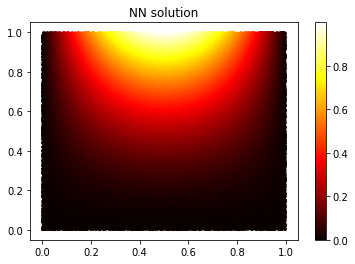
\includegraphics[width=0.8\linewidth]{images/NN_Jax_PDE8_files_elu/NN_Jax_PDE8_20_0.png}
    %\caption{A subfigure}
    \label{fig:sub2}
\end{subfigure}
\newline
\begin{subfigure}{.45\textwidth}
    \centering
    \includegraphics[width=.8\linewidth]{images/NN_Jax_PDE8_files_elu/NN_Jax_PDE8_22_0.png}
    %\caption{A subfigure}
    \label{fig:sub3}
    \end{subfigure}
\begin{subfigure}{.45\textwidth}
    \centering
    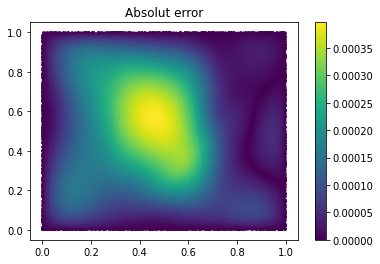
\includegraphics[width=.8\linewidth]{images/NN_Jax_PDE8_files_elu/NN_Jax_PDE8_24_0.png}
    %\caption{A subfigure}
    \label{fig:sub4}
\end{subfigure}
\caption{Results using Jax and elu}
\label{fig:test}
\end{figure}

\vspace{-0.5cm}
\subsection{Analysis}
According to the results obtained, the elu activation function takes longer to converge using the same parameters. Also, it is observed that the hyperbolic tangent provided a smaller absolute error for the same number of iterations.
\newpage

\section{TensorFlow approach}
\subsection{TensorFlow library}
\subsection{Solving with tanh}



\subsection{Solving with sigmoid}



\subsection{Solving with elu}


\subsection{Analysis}


\section{PyTorch}
\subsection{PyTorch library}



\subsection{Solving with tanh}



\subsection{Solving with sigmoid}



\subsection{Solving with elu}




\subsection{Analysis}

\chapter{Model}
\label{chapter4}
\section{Arcachon basin}
To do the simulation it is necessary to choose a location that has a lot of data available and a favorable geography, so we chose the Arcachon basin to do our simulation. The figure below shows the topology and bathymetry of this region.
The dataset was obtained from Shom France and OpenTopoData.
\vspace*{-0.85cm}
\begin{figure}[h]
    \hspace*{-1.5cm}
    \begin{subfigure}{0.5\textwidth}
        \centering
        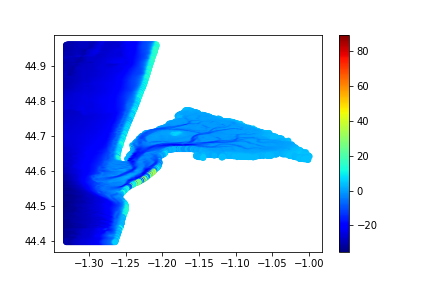
\includegraphics[scale=0.5]{images/Mesh/Mar_data.png}
        \caption{Bathymetry}
        \label{fig:sub1}
    \end{subfigure}%
    \hspace*{-2.7cm}
    \begin{subfigure}{0.5\textwidth}
        \centering
        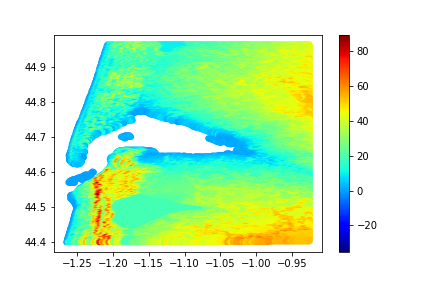
\includegraphics[scale=0.5]{images/Mesh/Topo_data.png}
        \caption{Topography}
        \label{fig:sub2}
    \end{subfigure}%
    \hspace*{-2.7cm}
    \begin{subfigure}{0.5\textwidth}
        \centering
        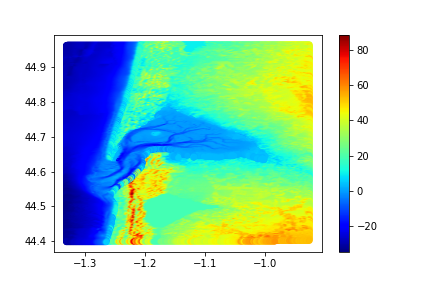
\includegraphics[scale=0.5]{images/Mesh/Topo_Mar_data.png}
        \caption{Topography and bathymetry}
        \label{fig:sub3}
    \end{subfigure}%
    \caption{Real datas for topography and bathymetry, on scale is the depth in meters}
    \label{fig:test}
    \end{figure}

\vspace{-0.75cm}
\section{Our approach}
With the data obtained from the topology and topography of this region, the delaunay method from the PyVista library was used to make the mesh. However, due to the way the data is collected in real life, there are very sharp variations in the height of the relief.
Thus, it is necessary to smooth these aspects, for this, we used the k-nearest neighbors (k-NN) with k=7 to make a mean and update the depth for each element in order to obtain a more regular structure. The figure below shows the mesh obtained for the dataset mentioned before.
\begin{figure}[h]
\begin{subfigure}{.5\textwidth}
    \centering
    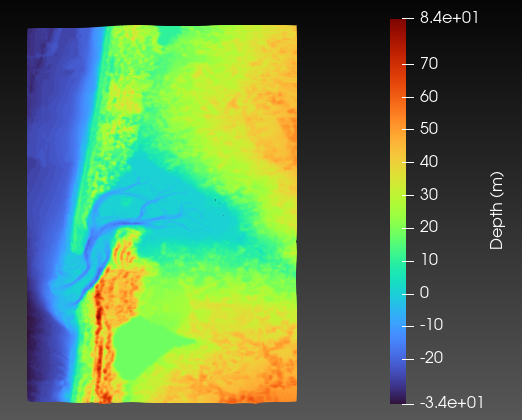
\includegraphics[width=0.7\linewidth]{images/Mesh/mesh_wireframe1.png}
    \caption{Topography and bathymetry}
    \label{fig:sub1}
\end{subfigure}%
\begin{subfigure}{0.6\textwidth}
    \centering
    \includegraphics[width=0.8\linewidth]{images/Mesh/mesh_wireframe.png}
    \caption{Wireframe}
    \label{fig:sub2}
\end{subfigure}%
\caption{Arcachon basin mesh}
\label{fig:test}
\end{figure}

\vspace{-0.75cm}
\section{Parallel processing}
The obtained structure has about 280000 elements and according to the simulations performed on chapter \ref{chapter3}, a very high number of loops will be required for the neural network to provide a good solution. However, due to the dimensions of the Mesh, the computational cost is very high, so a different approach is needed to do the simulation.
A very effective way to do this is to use parallel computing, i.e. the domain is divided into several subdomains that will be processed in different cores so that the same task is divided into small subtasks to speed up the final operation. 
So at each step of the main loop the neural net is put to train in the sub-domains, and then at the end of each loop the performance of the net is evaluated.
This procedure is described in the pseudo-code below.
\begin{algorithm}[H]
    \caption*{Gradient descent with parallel computing}
    \hspace*{\algorithmicindent} \textbf{Input}  NN\_parametres, p the number of simultaneous subtasks, loss\_function\\
    \hspace*{\algorithmicindent} \textbf{Output} new parametres
    \begin{algorithmic}
    \STATE repeat until convergence
        \bindent 
        \STATE get a training set and divide it into p-subsets with the same number of elements 
        \FOR {each n-processor}
            \STATE evaluate loss\_function of the n-subset
        \ENDFOR
        \STATE concatenate the p-set values obtained in the same training set order
        \STATE make gradient descent and update the parametres  
        \eindent
    \end{algorithmic}
    \end{algorithm}
    
\begin{itemize}
    \item To do this in Python we can use vmap function of Jax library to vectorize the gradient descent
\end{itemize}

\section{Mild slope equation}
\chapter{Simulation}
\label{chapter5} 



\chapter{Discussion of the results}
\label{chapter6} 




\chapter{Conclusion}
\label{ch:Conclusion} 

\section{Conclusion}

\section{Perspectives for new works and future improvements}

%\input{annexes.tex}
\chapter*{Bibliography}
\addcontentsline{toc}{part}{Bibliography}
\rhead{\nouppercase{Bibliography}}




%récupérer les citation avec "/footnotemark"


%choix du style de la biblio
\bibliographystyle{plain}
%inclusion de la biblio
\bibliography{bibliographie}
%voir wiki pour plus d'information sur la syntaxe des entrées d'une bibliographie


\end{document}
